\tikzset{every picture/.style={line width=0.75pt}} %set default line width to 0.75pt        

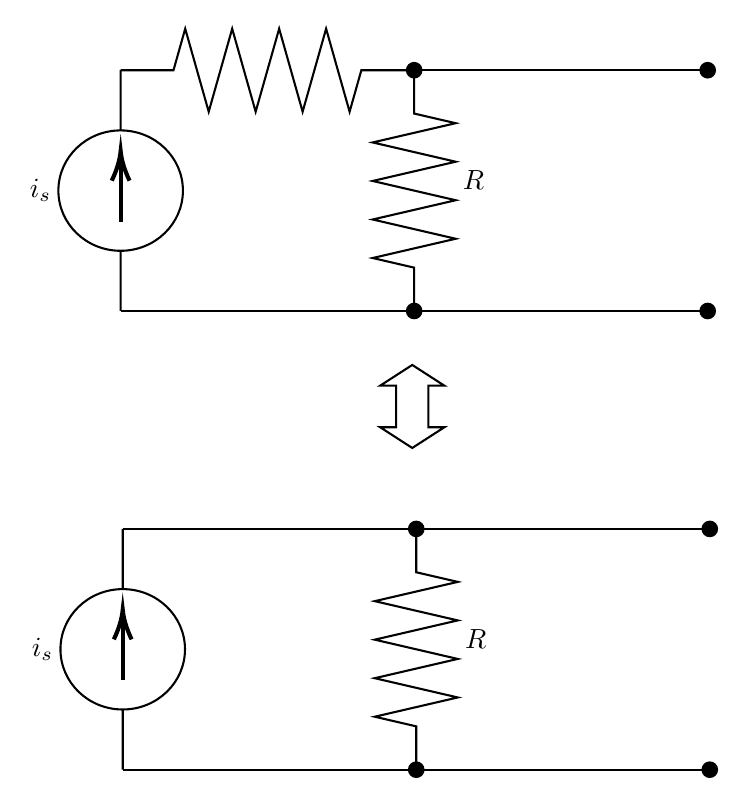
\begin{tikzpicture}[x=0.75pt,y=0.75pt,yscale=-1,xscale=1]
%uncomment if require: \path (0,642); %set diagram left start at 0, and has height of 642

%Shape: Output [id:dp8116510159532362] 
\draw   (196,61) .. controls (212.57,61) and (226,73.98) .. (226,90) .. controls (226,106.02) and (212.57,119) .. (196,119) .. controls (179.43,119) and (166,106.02) .. (166,90) .. controls (166,73.98) and (179.43,61) .. (196,61) -- cycle (196,32) -- (196,61) (196,148) -- (196,119) ;
%Straight Lines [id:da6552464425005597] 
\draw    (337.42,148) -- (196,148) ;
%Shape: Resistor [id:dp24941567689512412] 
\draw   (337.42,32) -- (337.42,52.88) -- (357.42,57.52) -- (317.42,66.8) -- (357.42,76.08) -- (317.42,85.36) -- (357.42,94.64) -- (317.42,103.92) -- (357.42,113.2) -- (317.42,122.48) -- (337.42,127.12) -- (337.42,148) ;
%Straight Lines [id:da8874958135805817] 
\draw    (478.84,32) -- (337.42,32) ;
%Straight Lines [id:da8322318838437468] 
\draw    (478.84,148) -- (337.42,148) ;
%Shape: Circle [id:dp9559322309363003] 
\draw  [fill={rgb, 255:red, 0; green, 0; blue, 0 }  ,fill opacity=1 ] (333.92,32) .. controls (333.92,30.07) and (335.49,28.5) .. (337.42,28.5) .. controls (339.35,28.5) and (340.92,30.07) .. (340.92,32) .. controls (340.92,33.93) and (339.35,35.5) .. (337.42,35.5) .. controls (335.49,35.5) and (333.92,33.93) .. (333.92,32) -- cycle ;
%Shape: Circle [id:dp9638608503252815] 
\draw  [fill={rgb, 255:red, 0; green, 0; blue, 0 }  ,fill opacity=1 ] (333.92,148) .. controls (333.92,146.07) and (335.49,144.5) .. (337.42,144.5) .. controls (339.35,144.5) and (340.92,146.07) .. (340.92,148) .. controls (340.92,149.93) and (339.35,151.5) .. (337.42,151.5) .. controls (335.49,151.5) and (333.92,149.93) .. (333.92,148) -- cycle ;
%Shape: Circle [id:dp33331887939722527] 
\draw  [fill={rgb, 255:red, 0; green, 0; blue, 0 }  ,fill opacity=1 ] (475.34,32) .. controls (475.34,30.07) and (476.91,28.5) .. (478.84,28.5) .. controls (480.78,28.5) and (482.34,30.07) .. (482.34,32) .. controls (482.34,33.93) and (480.78,35.5) .. (478.84,35.5) .. controls (476.91,35.5) and (475.34,33.93) .. (475.34,32) -- cycle ;
%Shape: Circle [id:dp8407733787615332] 
\draw  [fill={rgb, 255:red, 0; green, 0; blue, 0 }  ,fill opacity=1 ] (475.34,148) .. controls (475.34,146.07) and (476.91,144.5) .. (478.84,144.5) .. controls (480.78,144.5) and (482.34,146.07) .. (482.34,148) .. controls (482.34,149.93) and (480.78,151.5) .. (478.84,151.5) .. controls (476.91,151.5) and (475.34,149.93) .. (475.34,148) -- cycle ;
%Straight Lines [id:da7948900801514314] 
\draw [line width=1.5]    (196,105) -- (196,74) ;
\draw [shift={(196,71)}, rotate = 90] [color={rgb, 255:red, 0; green, 0; blue, 0 }  ][line width=1.5]    (14.21,-4.28) .. controls (9.04,-1.82) and (4.3,-0.39) .. (0,0) .. controls (4.3,0.39) and (9.04,1.82) .. (14.21,4.28)   ;
%Shape: Resistor [id:dp5308729023299701] 
\draw   (196,32) -- (221.46,32) -- (227.11,12) -- (238.43,52) -- (249.74,12) -- (261.05,52) -- (272.37,12) -- (283.68,52) -- (294.99,12) -- (306.31,52) -- (311.97,32) -- (337.42,32) ;
%Shape: Output [id:dp7710382379360781] 
\draw   (197,282) .. controls (213.57,282) and (227,294.98) .. (227,311) .. controls (227,327.02) and (213.57,340) .. (197,340) .. controls (180.43,340) and (167,327.02) .. (167,311) .. controls (167,294.98) and (180.43,282) .. (197,282) -- cycle (197,253) -- (197,282) (197,369) -- (197,340) ;
%Straight Lines [id:da9153416012919677] 
\draw    (338.42,369) -- (197,369) ;
%Shape: Resistor [id:dp14815855532060218] 
\draw   (338.42,253) -- (338.42,273.88) -- (358.42,278.52) -- (318.42,287.8) -- (358.42,297.08) -- (318.42,306.36) -- (358.42,315.64) -- (318.42,324.92) -- (358.42,334.2) -- (318.42,343.48) -- (338.42,348.12) -- (338.42,369) ;
%Straight Lines [id:da012078022892691775] 
\draw    (479.84,253) -- (364,253) -- (338.42,253) ;
%Straight Lines [id:da6929066887104642] 
\draw    (479.84,369) -- (338.42,369) ;
%Shape: Circle [id:dp04969927612649516] 
\draw  [fill={rgb, 255:red, 0; green, 0; blue, 0 }  ,fill opacity=1 ] (334.92,253) .. controls (334.92,251.07) and (336.49,249.5) .. (338.42,249.5) .. controls (340.35,249.5) and (341.92,251.07) .. (341.92,253) .. controls (341.92,254.93) and (340.35,256.5) .. (338.42,256.5) .. controls (336.49,256.5) and (334.92,254.93) .. (334.92,253) -- cycle ;
%Shape: Circle [id:dp5802490903591384] 
\draw  [fill={rgb, 255:red, 0; green, 0; blue, 0 }  ,fill opacity=1 ] (334.92,369) .. controls (334.92,367.07) and (336.49,365.5) .. (338.42,365.5) .. controls (340.35,365.5) and (341.92,367.07) .. (341.92,369) .. controls (341.92,370.93) and (340.35,372.5) .. (338.42,372.5) .. controls (336.49,372.5) and (334.92,370.93) .. (334.92,369) -- cycle ;
%Shape: Circle [id:dp15986570011337475] 
\draw  [fill={rgb, 255:red, 0; green, 0; blue, 0 }  ,fill opacity=1 ] (476.34,253) .. controls (476.34,251.07) and (477.91,249.5) .. (479.84,249.5) .. controls (481.78,249.5) and (483.34,251.07) .. (483.34,253) .. controls (483.34,254.93) and (481.78,256.5) .. (479.84,256.5) .. controls (477.91,256.5) and (476.34,254.93) .. (476.34,253) -- cycle ;
%Shape: Circle [id:dp4850989283457816] 
\draw  [fill={rgb, 255:red, 0; green, 0; blue, 0 }  ,fill opacity=1 ] (476.34,369) .. controls (476.34,367.07) and (477.91,365.5) .. (479.84,365.5) .. controls (481.78,365.5) and (483.34,367.07) .. (483.34,369) .. controls (483.34,370.93) and (481.78,372.5) .. (479.84,372.5) .. controls (477.91,372.5) and (476.34,370.93) .. (476.34,369) -- cycle ;
%Straight Lines [id:da5050251286211078] 
\draw [line width=1.5]    (197,326) -- (197,295) ;
\draw [shift={(197,292)}, rotate = 90] [color={rgb, 255:red, 0; green, 0; blue, 0 }  ][line width=1.5]    (14.21,-4.28) .. controls (9.04,-1.82) and (4.3,-0.39) .. (0,0) .. controls (4.3,0.39) and (9.04,1.82) .. (14.21,4.28)   ;
%Up Down Arrow [id:dp8919694665652462] 
\draw   (321,184) -- (336.5,174) -- (352,184) -- (344.25,184) -- (344.25,204) -- (352,204) -- (336.5,214) -- (321,204) -- (328.75,204) -- (328.75,184) -- cycle ;
%Straight Lines [id:da32870699744056053] 
\draw    (338.42,253) -- (222.58,253) -- (197,253) ;

% Text Node
\draw (164,90) node [anchor=east] [inner sep=0.75pt]   [align=left] {$\displaystyle i_{s}$};
% Text Node
\draw (359.42,79.08) node [anchor=north west][inner sep=0.75pt]   [align=left] {$\displaystyle R$};
% Text Node
\draw (165,311) node [anchor=east] [inner sep=0.75pt]   [align=left] {$\displaystyle i_{s}$};
% Text Node
\draw (360.42,300.08) node [anchor=north west][inner sep=0.75pt]   [align=left] {$\displaystyle R$};


\end{tikzpicture}
